\newpage
\section*{PROVIDE AN ADMINISTRATION API}

%The system has to offer the possibility of different administration possibilities, as e.g. a regular %performance check, creation of a new user or a re-start in the case of problems, but also the signalling of a %critical condition. 
%The system has to provide an API (application programming interface) that allows the system administrator to automate system administration tasks. Examples of such tasks are: a regular performance check, creation of a new user or a re-start in the case of problems, but also the signaling of a critical condition.  
The system to be built includes the possibilities of being configurable, whereby configuration files alone are not sufficient. These configurations are often administered by special employees, like application administrators, and not the core-users of the system itself.  

\begin{center}
\ding{118} \ding{118} \ding{118}
\end{center}

\textbf{If the administrative interface is a GUI, many of the standard administration tasks can not be automated. Repetitive tasks have to be completed again and again, which leads to a high frustration of the administrators. It also can be hard to get remote access to such a GUI.}\\

\textit{Unexpected usage.} System administrators have their own ways of organizing their administration tasks. The strive to automate many parts, often in unexpected ways, and a GUI is minimizing the possibilities of doing so.\\

\textit{Admin OS vs. System OS.} The operating systems which admins are using for their administration tasks often differ from the OS the application to be administered is running on. Providing an GUI as administrative interface often means that this GUI is only executable on certain OS's, which certainly restricts system administrators in an unnecessary way.

\begin{center}
\ding{118} \ding{118} \ding{118} 
\end{center}

\textbf{Therefore: Provide an API for all required administration functionality. Make this API available, easily accessible and well documented, so that admins can automate administrative tasks and integrate it easily in the administration processes.}\\

\textit{Solution in more detail.}

\textit{Consequences - first positive and then negative, relate these also to the forces}

Offering an API for the administrator provides much more flexibility to the system administrators for administering the systems in the way they think fits best. It gives them enough freedom to integrate the administration in existing processes.

Tools for automation can make use of the administration functionality if they can connect to the provided API. The right API helps to automate tasks that are part of a new employee account creation process. \cite{Limoncelli2011a}.

% negative consequences
There might be some security issues when exposing administrative features. Making use of a {\sc Proxy} \cite{Gamma95} can help here. The {\sc Proxy} can include an authentication mechanism and block all unauthorized access attempts. Make new diagram here including the proxy and authentication (relate to applicable authentication patterns here).

If the system evolves, then also the API is likely to change which might require adaptations the system developers are not aware of. TODO: The question is how to minimize the effect of system changes on the administrative API?

Providing an API might require a good documentation, whereas an administrative GUI can be more intuitive and self-explaining. For example: an API might require the correct spelling of user roles which need to be assigned to new users. A GUI can offer a selection list including all user roles and possibly an extra explanation of these roles in an apart window section. This minimizes the need for extra documentation. The API should therefore include an extensive help, containing all information necessary for using the provided administration functionality. For the same reason the API should include a good exception handling including good error messages. \\

%\textit{Implementation details, referring back to negative consequences}

TODO: how to implement? Also refer to {\sc Service Layer} in Fowler book \cite{Fowler:2002:PEA:579257}. And {\sc Facade} \cite{Gamma95}.  

TODO: what are the components and roles involved in the implementation of these patterns? 

\begin{figure}[h]
\centering
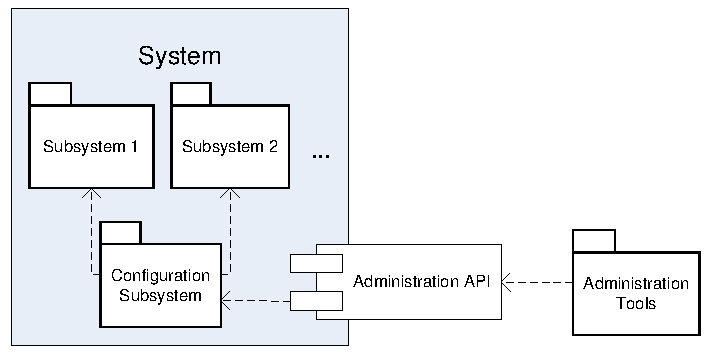
\includegraphics{patterns/provideAPIDiagram-01.pdf}
\caption{Solution structure}
\label{fig:provideAPIDiagram-01}
\end{figure}

TODO: say something about the way the API should/could be provided technically. Relate to force admin os vs system os.\\

\textit{One possibility of implementing this administrative API are the Java Management Extensions\footnote{\url{http://www.oracle.com/technetwork/java/javase/tech/javamanagement-140525.html}} (JMX). TODO: more }

\begin{center}
\ding{118} \ding{118} \ding{118} 
\end{center}

\textit{Rationale.}\\
Using this pattern will make the life of a system administrator more pleasant, especially in cross-platform situations, as it removes the platform-specific issues caused by a graphical administration interface. In combination with a cross-platform scripting language (e.g. Python, Ruby, TCL) this pattern shows its real strength as one can uniformly approach the administration API on any given platform.

